%
%%%%%%%%%%%%%%%%%%%%%%%%%%%%%%%%%%%%%%%%%%%%%%%%%%
% PLANTILLA EJERCICIOS DE HISTORIA DE LA MÚSICA I
% Este es un modelo para redactar los ejercicios
% 
% Pasos para cubrir la plantilla:
% 1) Realizar una copia de este modelo
% 2) Renombrar el archivo:
%		"HM1_Hoja(número).tex"
% 3) El número de Hoja debe ser correlativo
% 
%%%%%%%%%%%%%%%%%%%%%%%%%%%%%%%%%%%%%%%%%%%%%%%%%%
%
% Esta plantilla es para crear ejercicios de esta materia
% Se recomienda crear un archivo por cada tema
% Descomentar según se necesite utilizar un modelo de ejercicio u otro
% Clase de documento:
\documentclass[letterpaper,12pt,notitlepage,spanish]{article}
%
% Archivo externo de configuración
% --------------------------------
% Seleccionar o idioma:
%%%%%%%%%%%%%%%%%%%%%%%%%%%%%%%%%%%%%%%%%%%
%% ---------- MODELO EJERCICIOS ---------- 
%% MATERIA: HISTORIA
%% CURSO: 
%% AÑO ACADÉMICO: 
%% CENTRO: 
%%%%%%%%%%%%%%%%%%%%%%%%%%%%%%%%%%%%%%%%%%%
%% 
%% MODELO PARA REDACTAR EJERCICIOS
%% ===============================
%% 
%% Clase de documento
%% ------------------
%\documentclass[letterpaper,12pt,notitlepage,spanish]{article}
%\documentclass[12pt,a4paper,notitlepage]{article}
%
% Márgenes de documento
% ---------------------
\usepackage[left=2.0cm, right=2.0cm, lines=45, top=2.5cm, bottom=2.0cm]{geometry}
%
% Paquetes necesarios
% -------------------
\usepackage[utf8]{inputenc} % acentos en ES
\usepackage[spanish,activeacute, es-tabla]{babel}
\usepackage{enumerate} % entornos de listas
\usepackage{multicol}  % varias columnas texto
\usepackage{fancyhdr}  % encabezado personalizado
\usepackage{fancybox}  % entornos con cajas
\usepackage{pdfpages}  % páginas pdf
%
\usepackage{lipsum} % generar texto aleatorio "loren ipsum"
\usepackage{environ} 
\usepackage{probsoln} % paquete para soluciones
%\showanswers % para mostrar soluciones
%
%Esto es lo importante. Ponemos la solución al margen.
\NewEnviron{solutionnew}{%
%  \leavevmode\marginpar{\raggedright\footnotesize \textbf{Solución:}\\ \BODY}
%  \textbf{Solución:}\\ \BODY} % sol. con salto de liña
  \small{Solución:} \BODY} % sol. na mesma liña
  {}
\renewenvironment{solution}{\solutionnew}{\endsolutionnew}
%
% FIGURAS EN COLUMNAS:
\newenvironment{Figura}
  {\par\medskip\noindent\minipage{\linewidth}}
  {\endminipage\par\medskip}
% ---
%
% Lineas de encabezado y pié
% --------------------------
\renewcommand{\headrulewidth}{0.5pt}
%\renewcommand{\headrulewidth}{1.0pt}
\renewcommand{\footrulewidth}{0.5pt}
%\renewcommand{\footrulewidth}{1.0pt}
\pagestyle{fancy} % estilo de página
%
% Recuadros y figuras
% -------------------
\newcommand\Loadedframemethod{TikZ}
\usepackage[framemethod=\Loadedframemethod]{mdframed}
\usepackage{tikz}
\usetikzlibrary{calc,through,backgrounds}
\usetikzlibrary{matrix,positioning}
%Desssins geometriques
\usetikzlibrary{arrows}
\usetikzlibrary{shapes.geometric}
\usetikzlibrary{datavisualization}
\usetikzlibrary{automata} % LATEX and plain TEX
\usetikzlibrary{shapes.multipart}
\usetikzlibrary{decorations.pathmorphing} 
\usepackage{pgfplots}
\usepackage{physics}
\usepackage{titletoc}
\usepackage{mathpazo} 
\usepackage{algpseudocode}
\usepackage{algorithmicx} 
\usepackage{bohr} 
\usepackage{xlop} 
\usepackage{bbding} 
%\usepackage{minibox} 
% Texto árabe
\usepackage{mathdesign}
\usepackage{bbding} 
% --
% Tipograía:
% ----------
% Fuente HEURÍSTICA (cómoda de leer)
%\usepackage{heuristica}
% Fuente LIBERTINE (cómoda para apuntes)
\usepackage{libertineRoman}
%\usepackage[proportional]{libertine}
% Fuente ROMANDE (estilo antiguo pero no muy cómoda)
%\usepackage{romande} %
% 
% Encabezado y pié de página (textos)
% -----------------------------------
% Modelo 1:
% ---------
% texto de encabezado izquierda:
%\lhead{\normalfont{Historia de la Música I}}
% texto encabezado centro:
%\chead{\textbf{Ejercicios}}
% texto de encabezado derecha:
%\rhead{\normalfont{curso: 2020/2021}}
% texto pié izquierdo:
%\lfoot{\small{\textit{}}}
% texto pié centrado:
%\cfoot{\textsc{Pág. \thepage }}
% texto pié derecho
%\rfoot{\textit{Pr. $\mathcal{A}$.Kaal}}
% ----------
% Modelo 2:
% ---------
% Encabezado y pié de página (textos)
% -----------------------------------
% texto de encabezado izquierda:
%
%\lhead{
%	\hrule
%	\vspace*{0.20cm}
%	\normalfont{Historia de la Música I}
%	\vspace*{0.10cm}
	%\hrule
%}
% texto encabezado centro:
%\chead{
%	\textbf{Cuestionario de Ejercicios}
%	\vspace*{0.08cm}}
% texto de encabezado derecha:
%\rhead{
%	\normalfont{curso: 2020/2021}
%	\vspace*{0.08cm}}
%
% texto pié izquierdo:
%\lfoot{
	%\begin{center}
		%\vspace*{0.20cm}
		%\hrule
		%\small{
		%Conservatorio Profesional de Música de Viveiro - Avda. da mariña s/n - (27850) Viveiro - Lugo
		%	}
	%\end{center}
%}
% texto pié centrado:
%\cfoot{
	%\vspace*{0.30cm}
	%\hrule
	%\vspace*{0.90cm}
%	\small{- Página \thepage -  }\\
	%\small{Conservatorio Profesional de Música de Viveiro}\\
	%\small{avda. da Mariña s/n}
%}

% ----------
% Modelo 3:
% ---------
% Encabezado y pié de página (textos)
% -----------------------------------
% texto de encabezado izquierda:
%
\lhead{
	\hrule
	\vspace*{0.20cm}
	\normalfont{Historia da Música I}
	\vspace*{0.10cm}
	%\hrule
}
% texto encabezado centro:
\chead{
	\textbf{CADERNO DE EXERCICIOS}
	\vspace*{0.08cm}}
% texto de encabezado derecha:
\rhead{
	\normalfont{curso: 2021/2022}
	\vspace*{0.08cm}}
%
% texto pié izquierdo:
%\lfoot{
	%\begin{center}
		%\vspace*{0.20cm}
		%\hrule
		%\small{
		%Conservatorio Profesional de Música de Viveiro - Avda. da mariña s/n - (27850) Viveiro - Lugo
		%	}
	%\end{center}
%}
% texto pié centrado:
\cfoot{
	%\vspace*{0.30cm}
	%\hrule
	%\vspace*{0.90cm}
	\small{- \thepage -  }\\
	%\small{Conservatorio Profesional de Música de Viveiro}\\
	%\small{avda. da Mariña s/n}
}

% --------
%=====================Algo setup
\algblock{If}{EndIf}
\algcblock[If]{If}{ElsIf}{EndIf}
\algcblock{If}{Else}{EndIf}
\algrenewtext{If}{\textbf{si}}
\algrenewtext{Else}{\textbf{sinon}}
\algrenewtext{EndIf}{\textbf{finsi}}
\algrenewtext{Then}{\textbf{alors}}
\algrenewtext{While}{\textbf{tant que}}
\algrenewtext{EndWhile}{\textbf{fin tant que}}
\algrenewtext{Repeat}{\textbf{r\'ep\'eter}}
\algrenewtext{Until}{\textbf{jusqu'\`a}}
\algcblockdefx[Strange]{If}{Eeee}{Oooo}
[1]{\textbf{Eeee} "#1"}
{\textbf{Wuuuups\dots}}

\algrenewcommand\algorithmicwhile{\textbf{TantQue}}
\algrenewcommand\algorithmicdo{\textbf{Faire}}
\algrenewcommand\algorithmicend{\textbf{Fin}}
\algrenewcommand\algorithmicrequire{\textbf{Variables}}
\algrenewcommand\algorithmicensure{\textbf{Constante}}% replace ensure by constante
\algblock[block]{Begin}{End}
\newcommand\algo[1]{\textbf{algorithme} #1;}
\newcommand\vars{\textbf{variables } }
\newcommand\consts{\textbf{constantes}}
\algrenewtext{Begin}{\textbf{debut}}
\algrenewtext{End}{\textbf{fin}}
%================================
%================================

\setlength{\parskip}{1.25cm}
\setlength{\parindent}{1.25cm}
\tikzstyle{titregris} =
[draw=gray,fill=gray, shading = exersicetitle, %
text=gray, rectangle, rounded corners, right,minimum height=.3cm]
\pgfdeclarehorizontalshading{exersicebackground}{100bp}
{color(0bp)=(green!40); color(100bp)=(black!5)}
\pgfdeclarehorizontalshading{exersicetitle}{100bp}
{color(0bp)=(red!40);color(100bp)=(black!5)}
\newcounter{exercise}
%\renewcommand*\theexercise{exercice \textbf{Ejercicio}~n\arabic{exercise}} % CASTELÁN
\renewcommand*\theexercise{exercice \textbf{Exercicio}~n\arabic{exercise}} % GALEGO
\makeatletter
\def\mdf@@exercisepoints{}%new mdframed key:
\define@key{mdf}{exercisepoints}{%
\def\mdf@@exercisepoints{#1}
}
\mdfdefinestyle{exercisestyle}{%
outerlinewidth=1em,outerlinecolor=white,%
leftmargin=-1em,rightmargin=-1em,%
middlelinewidth=0.5pt,roundcorner=3pt,linecolor=black,
apptotikzsetting={\tikzset{mdfbackground/.append style ={%
shading = exersicebackground}}},
innertopmargin=0.1\baselineskip,
skipabove={\dimexpr0.1\baselineskip+0\topskip\relax},
skipbelow={-0.1em},
needspace=0.5\baselineskip,
frametitlefont=\sffamily\bfseries,
settings={\global\stepcounter{exercise}},
singleextra={%
\node[titregris,xshift=0.5cm] at (P-|O) %
{~\mdf@frametitlefont{\theexercise}~};
\ifdefempty{\mdf@@exercisepoints}%
{}%
{\node[titregris,left,xshift=-1cm] at (P)%
{~\mdf@frametitlefont{\mdf@@exercisepoints points}~};}%
},
firstextra={%
\node[titregris,xshift=1cm] at (P-|O) %
{~\mdf@frametitlefont{\theexercise}~};
\ifdefempty{\mdf@@exercisepoints}%
{}%
{\node[titregris,left,xshift=-1cm] at (P)%
{~\mdf@frametitlefont{\mdf@@exercisepoints points}~};}%
},
}
\makeatother


%%%%%%%%%

%%%%%%%%%%%%%%%
\mdfdefinestyle{theoremstyle}{%
outerlinewidth=0.01em,linecolor=black,middlelinewidth=0.5pt,%
frametitlerule=true,roundcorner=2pt,%
apptotikzsetting={\tikzset{mfframetitlebackground/.append style={%
shade,left color=white, right color=blue!20}}},
frametitlerulecolor=black,innertopmargin=1\baselineskip,%green!60,
innerbottommargin=0.5\baselineskip,
frametitlerulewidth=0.1pt,
innertopmargin=0.7\topskip,skipabove={\dimexpr0.2\baselineskip+0.1\topskip\relax},
frametitleaboveskip=1pt,
frametitlebelowskip=1pt
}
\setlength{\parskip}{0mm}
\setlength{\parindent}{10mm}
%\mdtheorem[style=theoremstyle]{ejercicio}{\textbf{Ejercicio}} % Castelán
\mdtheorem[style=theoremstyle]{ejercicio}{\textbf{Exercicio}} % Galego
%================Liste definition--numList-and alphList=============
\newcounter{alphListCounter}
\newenvironment
{alphList}
{\begin{list}
{\alph{alphListCounter})}
{\usecounter{alphListCounter}
\setlength{\rightmargin}{0cm}
\setlength{\leftmargin}{0.5cm}
\setlength{\itemsep}{0.2cm}
\setlength{\partopsep}{0cm}
\setlength{\parsep}{0cm}}
}
{\end{list}}
\newcounter{numListCounter}
\newenvironment
{numList}
{\begin{list}
{\arabic{numListCounter})}
{\usecounter{numListCounter}
\setlength{\rightmargin}{0cm}
\setlength{\leftmargin}{0.5cm}
\setlength{\itemsep}{0cm}
\setlength{\partopsep}{0cm}
\setlength{\parsep}{0cm}}
}
{\end{list}}
%
%
%% -- Fin del archivo de configuración  --
%% % Galego
%\input{../../Modelos/include/config-HM1ejercicios_ES.tex} % Castelán
% --------------------------------
\usepackage{graphicx}
\usepackage{hyperref}
%
%Ruta absoluta en formato tipo Unix (Linux, OsX)
%\graphicspath{{../../figures/}}
%
\setlength{\columnsep}{1cm} % separación entre columnas
\setlength{\columnseprule}{0.75pt}
\begin{document}
%
% DATOS DE HOJA DE EJERCICIOS
% ---------------------------
%
% TÍTULO DE LA HOJA DE EJERCICIOS:
%
\begin{center}
\Large{
3º Trimestre
} \\
\vspace*{0.5cm}
%
% NÚMERO DE HOJA:
%
%\normalsize % Número de hoja:
%(XVII - XVIII)
%\\
\vspace{1.10cm}
	\begin{flushleft}
	Nome e Apelidos: \hrulefill\\
	%\vspace*{0.50cm}
%		\begin{center}
%		\small{Instrucciones para realizar los ejercicios}\\		
%		\end{center}
%	\hrulefill \\
	%\vspace*{0.25cm}
%
%\small{ % INSTRUCCIONES:
%\texttt{Lee con atención y realiza con detenimiento, los siguientes ejercicios teniendo en cuenta lo que se indica en cada uno. \\
%}} % fin instrucciones.
%
	\vspace*{0.25cm}		
 	\end{flushleft}
\end{center}

% ------------------------------------
% ESPACIO PARA REDACTAR OS EXERCICIOS:
% ------------------------------------ 
% CABECEIRA EXERCICIOS:
\input{cabeceira-exercicios.txt}
% EXERCICIO 1.- Contextualización Renacemento
% -------------------------------------------
%% EXERCICIOS PARA INCLUÍR DENTRO DO CADERNO DE EXERCICIOS %%
%
% EXERCICIO.- RENACEMENTO: Contextualización
%
\section{A música no <<Renacemento>> } 
%
% -------------------------------
% BANCO DE PREGUNTAS DE HISTORIA
% -------------------------------
%
% Tema 4.- MÚSICA NO RENACEMENTO
% ------------------------------
% Comentario.- 
%
% EXERCICIO.- 
% -------------------------------------
%\newproblem{T4RENA-01}{
%
Adoita situarse a orixe do Renacemento como fenómeno cultural e artístico, nas cidades italianas do norte e en Roma, xunto coas de Flandes e Países Baixos e, por tanto, relacionado con áreas de forte desenvolvemento urbano e comercial. Desde estes focos iniciais, o Renacemento estenderíase a toda Europa paulatinamente. A cronoloxía clásica distingue entre \href{http://es.wikipedia.org/wiki/Quattrocento}{\emph{quattrocento}} e \href{http://es.wikipedia.org/wiki/Cinquecento}{\emph{cinquecento}.}
%
\par
\vspace*{0.25cm}
%
\begin{ejercicio}[Periodización - Renacemento]
Lé con atención o seguinte texto e responde a cuestión.
%\begin{multicols}{2}
    \begin{quote}
    O concepto de \href{http://es.wikipedia.org/wiki/Renacimiento}{Renacemento} aparece para a historiografía da arte e da cultura en época tan distante como o século XIX. Este termo refírese á recuperación da cultura da \href{http://es.wikipedia.org/wiki/Antig\%C3\%BCedad_cl\%C3\%A1sica}{Antigüidade} \href{http://es.wikipedia.org/wiki/Antig\%C3\%BCedad_cl\%C3\%A1sica}{clásica} tras o longo período, supostamente escuro, que suporía a \href{http://es.wikipedia.org/wiki/Edad_Media}{Idade Media.} [\ldots] \\
    Efectivamente, os séculos XV e XVI trouxeron grandes cambios, así como a formación dalgúns dos principios estruturais que estiveron operativos na cultura europea até as revolucións burguesas dos séculos XVIII e XIX. De feito, basta lembrar que a historiografía fai comezar no século (\ldots) unha nova \href{http://es.wikipedia.org/wiki/Edad_Moderna}{Idade Moderna.}
\end{quote}
\begin{flushright}
 J.Jurado: \textit{Apuntamentos para a historia da música}
\end{flushright}
%
Tendo en conta a periodización que coñeces, a que século se está a referir o autor da cita? \ldots
\par
\vspace*{0.15cm}
    \begin{tabular}{c c c c}
        a) XIV & b) XV & c) XIII & d) XVI  \\
    \end{tabular}

%\end{multicols}
\end{ejercicio}
%}
% {a)}
% comentario da resposta:
%    \\ \small{Indica o comentario}
%


% --------------------------------------------
\subsection*{Trazos culturais do Renacemento}
%
% -----------------------------------------
% CUESTIÓN: TRAZOS DA CULTURA RENACENTISTA 
% -----------------------------------------
% Comentario.- 
%
%
% EXERCICIO.- 
% -------------------------------------
%\newproblem{T4RENA-02}{
%
Facendo unha síntese, podemos enunciar os trazos xerais da cultura do
Renacemento: 
\begin{multicols}{2}
Crecemento económico e demográfico: o Renacemento ve nacer os principios da economía capitalista (bancos, letras, crédito...). Paralelamente, obsérvase un crecemento das cidades e das clases que lle son propias: a burguesía. O propio concepto moderno de Estado alcanza a súa formulación nas obras de \href{http://es.wikipedia.org/wiki/Maquiavelo}{Maquiavelo.} A nivel social, a expansión das clases burguesas favoreceu a demanda dunha arte laica, en detrimento do protagonismo da arte relixioso que dominara o período anterior.
\par
Desenvolvemento científico e tecnolóxico, ilustrado pola revolución \href{http://es.wikipedia.org/wiki/Cop\%C3\%A9rnico}{copernicana} e a creatividade de personaxes como \href{http://es.wikipedia.org/wiki/Leonardo_da_Vinci}{Leonardo da Vinci.} sentan as bases do \href{http://es.wikipedia.org/wiki/M\%C3\%A9todo_cient\%C3\%ADfico}{método científico} e experimental que se desenvolve con forza e que abre a porta á ciencia moderna e á sociedade tecnolóxica.
\par
A nivel cultural pode falarse dun xiro fundamental coa invención da \href{http://es.wikipedia.org/wiki/Imprenta}{imprenta} a mediados do XV e as posibilidades de expansión de ideas que iso supón. O vigor das universidades e a circulación de información favoreceron a expansión do \href{http://es.wikipedia.org/wiki/Humanismo}{Humanismo.} O Humanismo comprende toda unha antropoloxía dentro da cal a persoa pasa a ocupar un lugar central como punto desde o que se observa e valora a realidade. O pensamento individual asume a responsabilidade de elaborar unha interpretación correcta do mundo mediante un medio crítico baseado na experimentación. O punto de vista crítico do Humanismo respecto diso dunha interpretación dogmática do mundo é, en boa parte, o desencadenamento da crise relixiosa e dos movementos protestantes do XVI.
\par
A creación artística será un dos aspectos máis rechamantes do período. En primeiro lugar polo novo concepto de arte: o artista xa non é un artesán ao servizo da inspiración divina, senón un creador que aspira ao status de home de ciencia. Poucos períodos da Historia de Occidente coñeceron un ritmo de produción de obras de arte tan intenso en calidade e cantidade como este, porque posta ao servizo da exaltación do poder persoal (príncipes, papas...) a creación artística convértese nun elemento de prestixio privilexiado, facendo do mecenado unha institución obrigada para calquera poderoso.\\
\par
\vspace*{0.25cm}
(J.Jurado \textit{Apuntamentos para a Historia da Música}. Ed. Dos Acordes. Vigo 2017.)
\\
%\hrulefill
%
\end{multicols}

\begin{ejercicio}[Trazos da cultura do Renacemento]
Realiza un resumo das principais características que consideras definen a cultura renacentista, tendo en conta o texto do Profesor Jurado. 
\par
\vspace*{9.5cm}
\end{ejercicio}
%}
% {a)}
% comentario da resposta:
%    \\ \small{Indica o comentario}
%


%\newpage
%
% EXERCICIO 2.- 
% -------------------------------------
%%% EXERCICIOS PARA INCLUÍR DENTRO DO CADERNO DE EXERCICIOS %%
%
% EXERCICIO.- ANÁLISE DA SECUENCIA: Dies irae
%
\section{Análise da secuencia <<Dies irae>>} \label{Intro}
%
Unha das secuencias máis coñecidas é o <<Dies irae>>, que no século XV empezouse a considerar parte da misa de defuntos, converténdose cara finais de século, nun movemento obrigado desta misa.

Para realizar a análise con partitura da audición desta secuencia, seguiremos os pasos indicados na analise de audición do <<Puer natus est>>  (ver o punto \ref{sec:Puer-natus} da páxina \pageref{sec:Puer-natus}); unha vez realizada a análise da partitura e escoita activa, completaremos os datos da obra.
\par
\vspace*{0.15cm}
%
% ----------------------
% Partitura de audición:
% ----------------------
\begin{figure}[h]
    \centering
    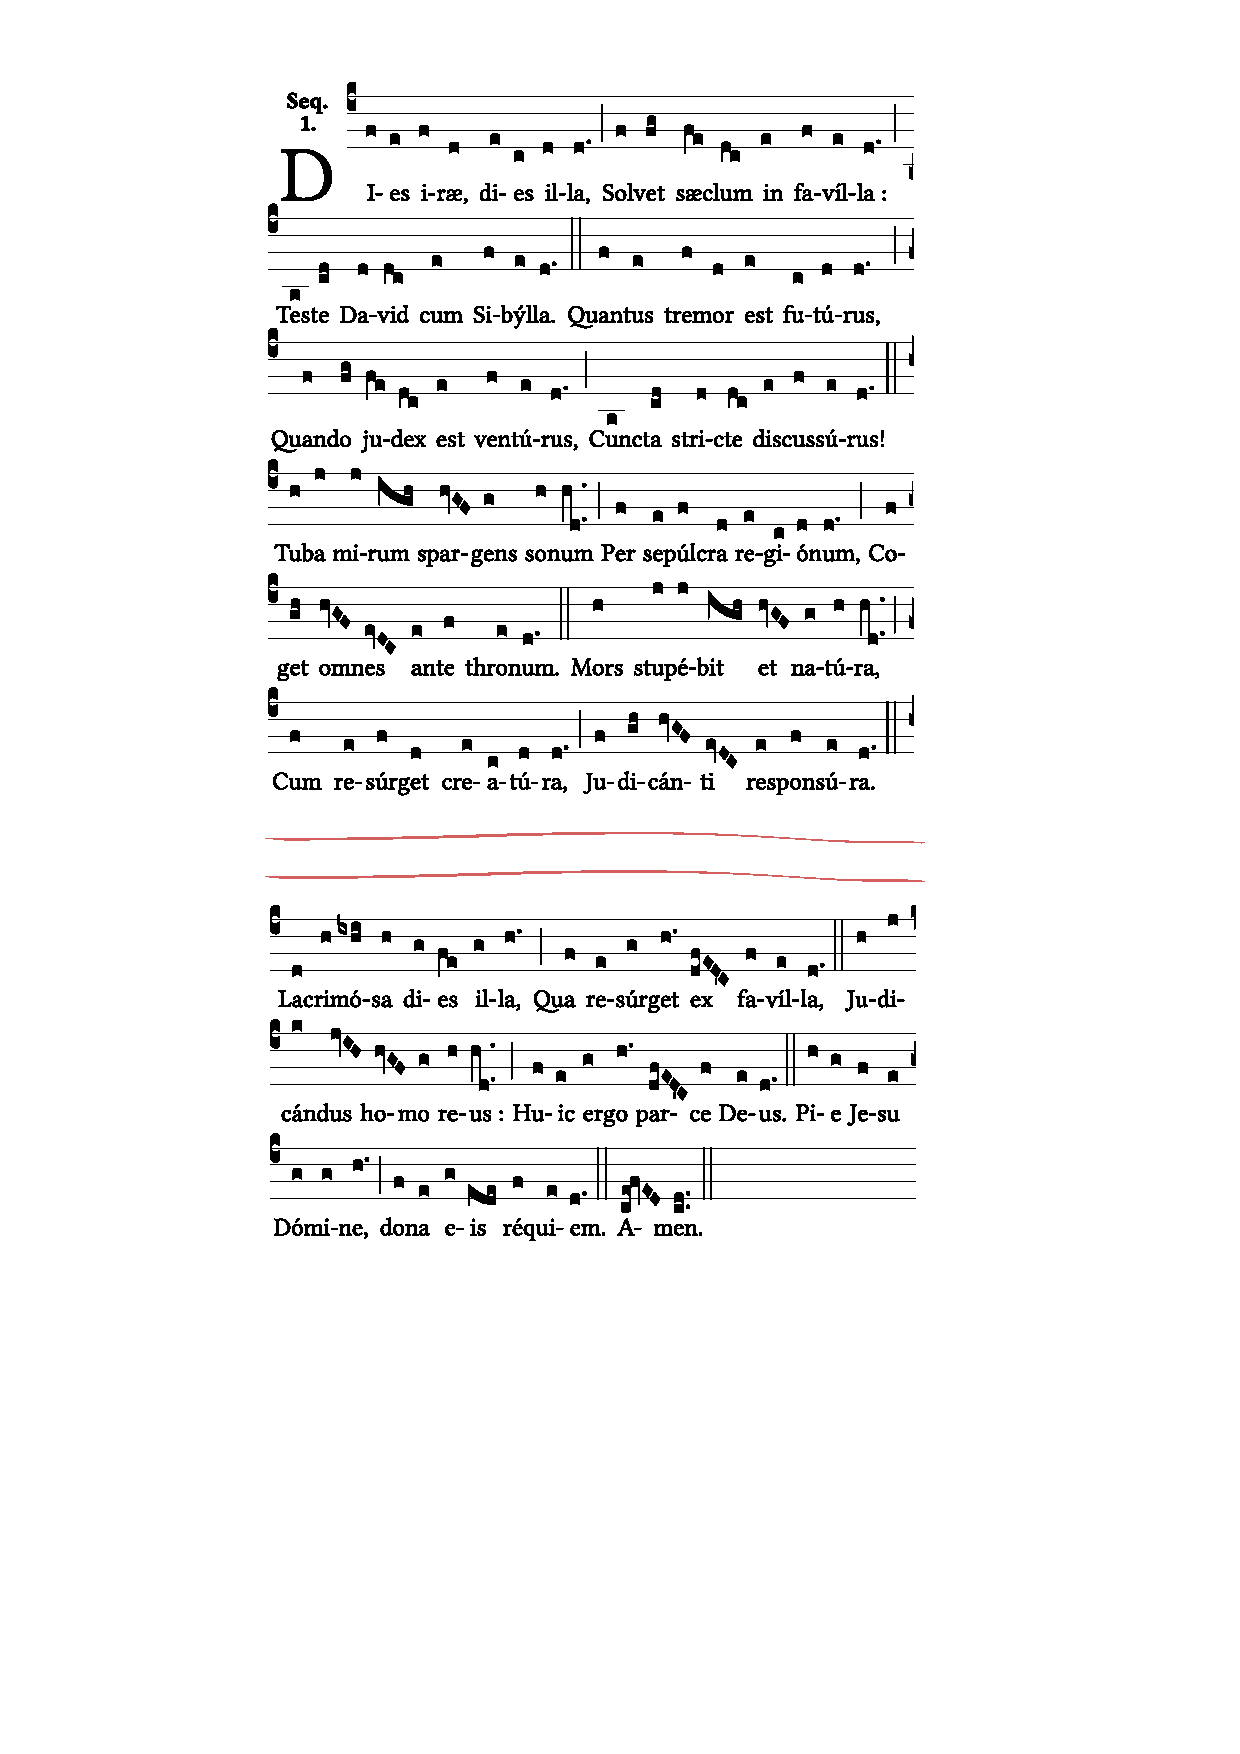
\includegraphics[width=0.60\textwidth]{ud-03/dies-irae-solesmes-cut.pdf}
    \caption{Secc. do inicio e fin do <<Dies irae>>}
    \label{fig:dies-irae}
\end{figure}
% -----------------------
%
%\par
%\vspace*{0.25cm}
% INTRODUCCIÓN
% TODO: Revisar !!
%
%Trátase dunha peza monódica con texto en latín, sen ritmo estruturado, de estilo silábico, con unha estrutura de repetición que se podería representar co seguinte esquema: a bb cc dd e. 
%A primeira frase cántase unha soa vez, pero a segunda, terceira e cuarta cántanse dúas veces con textos diferentes. A música é diferente para cada frase. Termina cunha pequena frase que se canta unha soa vez.

%Polo xeral estas pezas distínguense por ser silábicas e, sobre todo, ter frases de música que se repiten por pares. A maioría teñen unha soa frase ao principio e ao final, e pares de frases intermedias. 
%En qué consiste a repetición pareada?
%As frases en pares repiten a melodía, pero o texto cambia. A forma é a bb cc dd ee… nn. Moitas secuencias son pezas moi longas, por exemplo o dies irae, mentres que unhas poucas, como o victimae paschali laudes, son curtas.
%
%\subsection*{Análise da audición} 

\begin{multicols}{2}

%\begin{enumerate}[1.-]
%PUNTO NÚMERO 1: ESCOITAR A PEZA
%
%\subsubsection*{Paso no. 1: análise da partitura} \label{analise-partitura}
%
%No caso de análise dunha audición con partitura prestaremos atención a tódolos elementos formais que observamos na partitura (notación e demáis grafías); son os primeiros elementos a recoñecer a golpe de vista.
%Aqueles elementos que son descoñecidos ou non recoñecemos a simple vista, rodearémolos cun círculo para aclarar o seu significado.
%
%\subsubsection*{Paso no. 2: escoita activa} \label{escoita}
%
%Despois da observación e lectura e identificaremos os elementos formais por medio dunha escoita activa da obra.
%É moi importante identificar auditivamente todo o que observamos no paso \ref{analise-partitura}.
%A escoita activa, axudaranos a determinar a relación música-texto da obra neste caso.
%
%\subsubsection*{Paso no.3: datos da audición} \label{datos-audicion}
%
%Unha vez realizados os pasos \ref{analise-partitura} e \ref{escoita} prestaremos atención aos seguintes puntos.
%
    \begin{enumerate}[1.-]
% ANÁLISE DO RITMO DA OBRA:
        \item % RITMO
        \textbf{Ritmo}. Identificamos o ritmo, tendo en conta: pulso, indicacións de compás e outras indicacións dinámicas. 
        Neste caso, estamos ante un ritmo:
        \begin{enumerate}[a)]
            \item mensural 
            \item non mensural 
        \end{enumerate}
% ANÁLISE DA MELODÍA DA OBRA:
        \item %MELODÍA:
        \textbf{Melodía}. Tendo en conta a melodía, determinamos o modo, ámbito e estilo. Prestaremos atención ao perfil melódico e interválica, observando se hai grandes saltos ou mais ben discorre por graos conxuntos.
%        \begin{multicols}{2}
        \begin{enumerate}[a)]
            \item 
            Que intervalos se repiten con maior frecuencia? \dotfill
            \item 
            Cal é o maior intervalo que podemos atopar na peza? \dotfill
            \item
            Podemos afirmar que a melodía se move por graos \dotfill
        \end{enumerate}
%        \end{multicols}
        Vexamos a continuación o Modo, Ámbito e Estilo tendo en conta a melodía:
        \begin{itemize}
% ANÁLISE DO MODO:
            \item % MODO
            \textbf{Modo}.
        \begin{itemize}            
            \item 
            Identifica a clave \dotfill
            \item 
            Cal é a nota \textit{finalis}? \dotfill
            \item
            En que modo básico estamos? \dotfill
            \item
            Cal é a nota máis agura? \dotfill 
            \item
            Cal é a nota máis grave? \dotfill 
            \item
            Que intervalo forma coa final? \dotfill
            \item
            Cal é a nota tenor? \dotfill 
            \item
            En qué modo esta a obra? \dotfill
       \end{itemize}
% ANÁLISE DO ÁMBITO DA OBRA:
            \item % ÁMBITO
            \textbf{Ámbito}. \\
            Fixándonos na nota \textit{finalis} e na máis aguda:
                \begin{itemize}
                    \item
                    Que intervalo forman? \dotfill
                    \item
                    A melodía é de ámbito \dotfill
                \end{itemize}
            \item % ESTILO
            \textbf{Estilo do canto}. \\ Segundo a relación musica-texto, estamos ante un estilo:
                \begin{enumerate}[a)]
                  \item
                  Silábico \dotfill
                  \item
                  Neumático \dotfill
                  \item
                  Melismático \dotfill
                \end{enumerate}
        \end{itemize}
        \item % TIMBRE
        \textbf{Timbre}. \\
        Segundo as características da obra, debemos diferenciar as voces, instrumentos, formacións, agrupacións, ...
            \begin{itemize}
                \item 
                Que timbres recoñeces? \dotfill
                \item
                Polo tanto, trátase de \dotfill
            \end{itemize}
% ANÁLISE DA TEXTURA DA OBRA:
        \item %TEXTURA
        \textbf{Textura}. \\
        Polas características da obra, diferenciamos unha textura melódica \ldots 
            \begin{enumerate}[a)]
                \item 
                De escrita horizontal, monódica
                \item 
                De escrita horizontal, polifónica
            \end{enumerate}
% ANÁLISE DA FORMA DA OBRA
        \item %FORMA:
        \textbf{Forma}. \\
        Determinamos a forma segundo a extensión, textura e estrutura da obra. \\ 
        \par %Pregunta sobre as Formas
        A que tipo de forma, podemos dicir que se axusta esta obra?
        \begin{enumerate}[a)]
            \item 
            Forma vocal menor libre
            \item
            Forma vocal menor ternaria
            \item
            Forma vocal maior ternaria
            \item
            Forma instrumental menor ternaria
        \end{enumerate}
        \end{enumerate}
%    \end{multicols}
%
\end{multicols}
%\vspace*{0.25cm}
%
\subsubsection*{Clasificación no repertorio} 
Unha vez realizada a análise da audición, tendo en conta os datos obtidos, clasificaremos a obra tendo en conta sobre todo o ámbito e estilo.
%
% RESUMO DA AUDICIÓN DO EXERCICIO
%
\vspace*{0.5cm}
\begin{ejercicio}[Características principais da audición: <<Dies irae>>]
%\small{
%Redacta un breve comentario da obra. Ten en conta a análise feita:
%}

% ESPACIO PARA REDACTAR O COMENTARIO DA AUDICIÓN
%
%\small{Trátase dunha forma vocal menor, de estrutura ternaria; segundo o ámbito e estilo, obedece a un canto antifonal do propio da misa cantado a capella por un coro de voces masculinas; a textura monódica horizontal é propia do canto chá (Gregoriano) en estilo neumático na primeira sección e silábico na segunda, de ámbito reducido escrita no modo \textit{tetrardus auténtico} (VII)     }

        \vspace*{2.78cm}
\end{ejercicio}


%\newpage
%
% EXERCICIO 3.- 
% ------------------------------
%% -----------------------------------
% FICHAS DE AUDICIÓNS PARA COMPLETAR:
% -----------------------------------
\subsection*{Exercicio de audición sen partitura}
%
Escoita con atención as audicións propostas para este trimestre, completa as fichas e responde ás cuestións.
%
%
% AUDICIÓN 1.- NUPER ROSARUM FLORES
% ---------------------------------
% 
%
\vspace*{0.25cm}

\begin{ejercicio}[] 
%
Completa a ficha da obra proposta como exercicio de audición.
%
\begin{multicols}{2}
	\begin{enumerate}[1.-]
        \vspace*{0.3cm}
		\item
			Autor: \dotfill
			\vspace*{0.3cm}
		\item
			Obra:
			\begin{enumerate}[a)]
			    \item Título: \dotfill \vspace*{0.3cm}
			    \item Período: \dotfill \vspace*{0.3cm}
			    \item Forma: \dotfill \vspace*{0.3cm}
			    \item Timbre: \dotfill 			\vspace*{0.3cm}
			    \item Textura: \dotfill \vspace*{0.3cm}
			    \item Estilo: \dotfill \vspace*{0.3cm}
			    \item Xénero: \dotfill 
			    \vspace*{0.3cm}
			\end{enumerate}
	\end{enumerate}
\end{multicols}
	\begin{itemize}
%	    \item 
%Identifica a escola e xeración, á que podería pertencer o autor desta obra:
%    \vspace*{0.25cm}
    
%    \begin{tabular}{l l l l}
%        a) Franco-flamenca; $1^a$ xeración \\ 
%        b) Franco-flamenca; $2^a$ xeración \\
%        c) Franco-flamenca; $4^a$ xeración \\
%        d) Franco-flamenca; $3^a$ xeración \\
%    \end{tabular}
    
    \item
    Partindo dos datos dispoñibles na ficha de audición, realiza un breve comentario da obra.
    \vspace*{12cm}
	\end{itemize}

\end{ejercicio}
%
%%
% AUDICIÓN 2.- 
% ----------------------
%
\begin{ejercicio}[]
%
Completa a ficha da obra proposta como exercicio de audición.
%
\begin{multicols}{2}
	\begin{enumerate}[1.-]
        \vspace*{0.3cm}
		\item
			Autor: \dotfill
			\vspace*{0.3cm}
		\item
			Obra:
			\begin{enumerate}[a)]
			    \item Título: \dotfill \vspace*{0.3cm}
			    \item Período: \dotfill \vspace*{0.3cm}
			    \item Forma: \dotfill \vspace*{0.3cm}
			    \item Timbre: \dotfill \vspace*{0.3cm} 		
			    \item Textura: \dotfill \vspace*{0.3cm}
			    \item Estilo: \dotfill \vspace*{0.3cm}
			    \item Xénero: \dotfill \vspace*{0.3cm}
			\end{enumerate}
%		\item 
%		    Resume as principais características que definen a obra:
%			\vspace*{8.0cm}			

	\end{enumerate}
\end{multicols}
	\begin{itemize}
%	    \item 
%Identifica a escola e xeración, á que podería pertencer o autor desta obra:
%    \vspace*{0.25cm}
    
%    \begin{tabular}{l l l l}
%        a) Franco-flamenca; $1^a$ xeración \\ 
%        b) Franco-flamenca; $2^a$ xeración \\
%        c) Franco-flamenca; $4^a$ xeración \\
%        d) Franco-flamenca; $3^a$ xeración \\
%    \end{tabular}
    
    \item
    Partindo dos datos dispoñibles na ficha de audición, realiza un breve comentario da obra.
    \vspace*{14cm}
	\end{itemize}
\end{ejercicio}
%

%\newpage
%
% EXERCICIO 4.- 
% ---------------------------------
%%
% ----
\hideanswers % oculta respostas
%
% Cargamos os Exercicios:
% ----------------------

\loadallproblems[Tema3-GREGO]{../../Cuestions/Tema3-Canto-gregoriano.tex}

\loadallproblems[Tema3-GREGO1]{../../Cuestions/Tema3-Canto-gregoriano-expansion.tex} %
%\loadallproblems[Tema3-NOTA]{../../Cuestions/Tema3-Notacion-modal.tex} %
%\loadallproblems[Tema1-PENS]{../../Cuestions/Tema1-Pensamento.tex} %
%\loadallproblems[Tema1-RO]{../../Cuestions/Tema1-Roma.tex} %
%\loadrandomproblems[loops]{2}{loops}% aleatorios
%
% FOLLA EXERCICIOS: 
% -----------------
\begin{multicols}{2} % a 2 columnas
    \begin{enumerate}
%\useproblem{input}
    \foreachproblem[Tema3-GREGO]{\item\label{prob:\thisproblemlabel}\thisproblem}
    \foreachproblem[Tema3-GREGO1]{\item\label{prob:\thisproblemlabel}\thisproblem}
 %   \foreachproblem[Tema3-NOTA]{\item\label{prob:\thisproblemlabel}\thisproblem}
%    \foreachproblem[Tema1-PENS]{\item\label{prob:\thisproblemlabel}\thisproblem}
    \end{enumerate}
\end{multicols}
%
% SOLUCIONS:
% ----------
%\newpage
%\begin{multicols}{2}
%\showanswers
%\begin{itemize}
%\foreachdataset{\thisdataset}{%
%\foreachproblem[\thisdataset]{\item[\ref{prob:\thisproblemlabel}]\thisproblem}
%}
%\end{itemize}
%\end{multicols}
%\newpage
%
% EXERCICIO 5.- 
% ------------------------------------
%\input{Exercicio-A-Chantar-comentario.tex}
%\newpage
%
% EXERCICIO 6.- 
% -------------
%%
% ----
\hideanswers % oculta respostas
%
% Cargamos os Exercicios:
% ----------------------

\loadallproblems[Tema3-GREGO]{../../Cuestions/Tema3-Canto-gregoriano.tex}

\loadallproblems[Tema3-GREGO1]{../../Cuestions/Tema3-Canto-gregoriano-expansion.tex} %
%\loadallproblems[Tema3-NOTA]{../../Cuestions/Tema3-Notacion-modal.tex} %
%\loadallproblems[Tema1-PENS]{../../Cuestions/Tema1-Pensamento.tex} %
%\loadallproblems[Tema1-RO]{../../Cuestions/Tema1-Roma.tex} %
%\loadrandomproblems[loops]{2}{loops}% aleatorios
%
% FOLLA EXERCICIOS: 
% -----------------
\begin{multicols}{2} % a 2 columnas
    \begin{enumerate}
%\useproblem{input}
    \foreachproblem[Tema3-GREGO]{\item\label{prob:\thisproblemlabel}\thisproblem}
    \foreachproblem[Tema3-GREGO1]{\item\label{prob:\thisproblemlabel}\thisproblem}
 %   \foreachproblem[Tema3-NOTA]{\item\label{prob:\thisproblemlabel}\thisproblem}
%    \foreachproblem[Tema1-PENS]{\item\label{prob:\thisproblemlabel}\thisproblem}
    \end{enumerate}
\end{multicols}
%
% SOLUCIONS:
% ----------
%\newpage
%\begin{multicols}{2}
%\showanswers
%\begin{itemize}
%\foreachdataset{\thisdataset}{%
%\foreachproblem[\thisdataset]{\item[\ref{prob:\thisproblemlabel}]\thisproblem}
%}
%\end{itemize}
%\end{multicols}
%\newpage
%
% EXERCICIO 7.- 
% -------------
%\input{Exercicio-A-Chantar-comentario.tex}
%\newpage
%
% EXERCICIO 8.- 
% -------------
%\input{Exercicio-A-Chantar-comentario.tex}
%\newpage
%
% EXERCICIO 9.- 
% -------------
%\input{Exercicio-A-Chantar-comentario.tex}
%\newpage
%
% EXERCICIO 10.- 
% -------------
%\input{Exercicio-A-Chantar-comentario.tex}
%\newpage
\end{document}
%Fin de Hoja de ejercicios
%